\chapter{Resultados} %#{{{1
\label{chap:resultados}

\begin{epigraphs}
\qitem{ One important idea is that science is a means whereby learning is
achieved, not by mere theoretical speculation on the one hand, nor by the
undirected accumulation of practical facts on the other, but rather by a
motivated iteration between theory and practice.
}
{\---- \textsc{George E. P. Box, 1912-2013}}
\end{epigraphs}

A principal motivação desse trabalho é descrever, através de uma modelagem
matemática de agentes interagentes, o fenômeno social do aprendizado moral
e suas conexões com ideologia política, estratégia cognitiva e quantidade
informação moral obtida durante a infância e adolescência. Portanto, o
foco desse capítulo são os resultados computacionais que podem ser comparados
diretamente com algumas evidências experimentais relativas a esses assuntos.


\section{Ideologia política do agente Bayesiano} %#{{{2

Apesar dos agentes não apresentam ideologia política, nós podemos medir as
distribuições de opiniões sobre o \textit{zeitgeist} $P_S(h|\rho,\beta)$
no estado estacionário da fase 2 do modelo para uma sociedade em que todos
os agentes estão submetidos a um mesmo valor de $\beta$ e $\rho$ . Com
essa assinatura estatística, podemos comparar com a assinatura similar
obtida através dos dados do questionário sobre Fundamentos Morais para
cada filiação política, e encontrar a região de parâmetros do modelo que é mais
similar ao perfil estatístico das opiniões de pessoas com uma determinada
ideologia política.

\begin{figure}
    \centering
    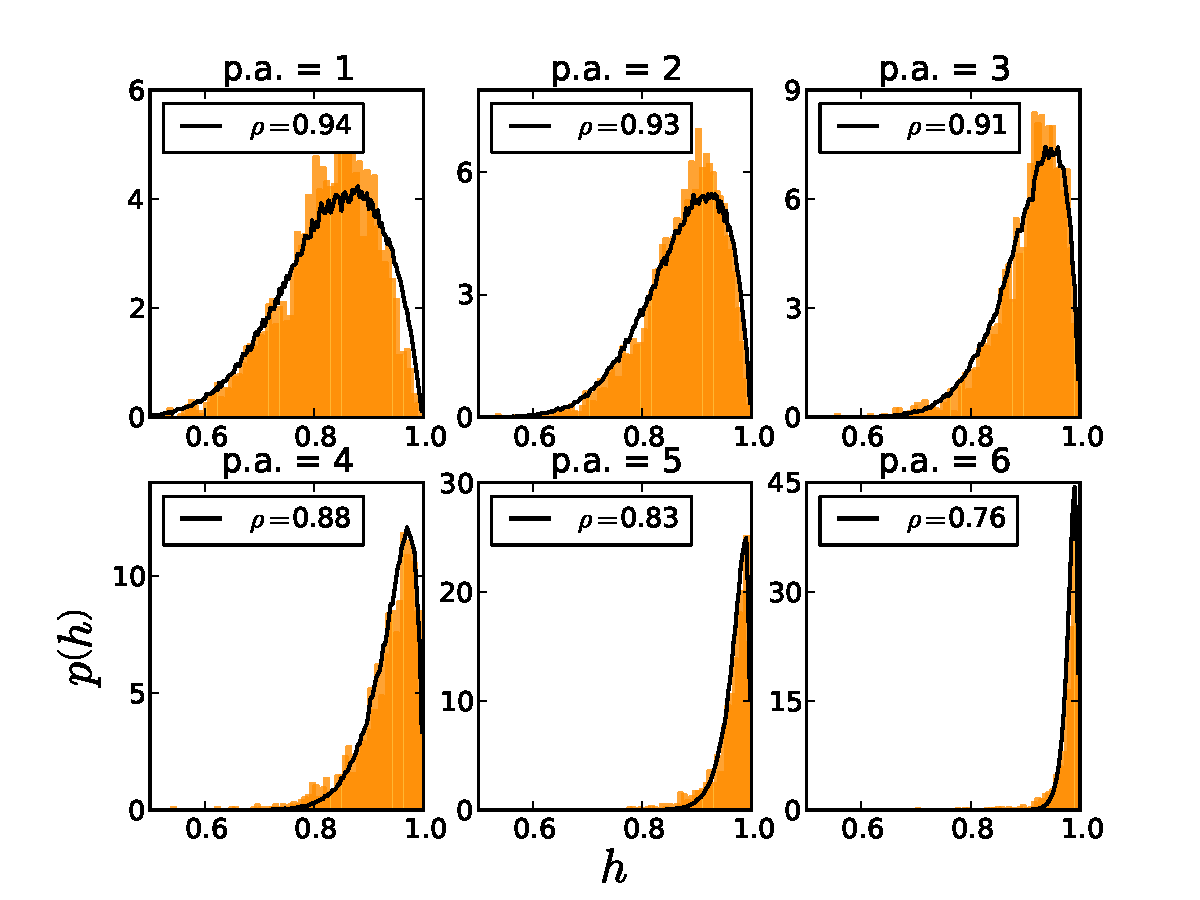
\includegraphics[scale=0.5]{Figures/hists_b38}
    \caption{
        Comparação entre os histogramas de opinião, em relação ao
        \textit{zeitgeist}, obtidos através de simulação (linhas pretas)
        e obtidos através do questionário sobre fundamentos morais (caixas
        laranjas). O valor do parâmetro de pressão social usado nesses
        resultado foi de $\log(\beta)=3,8$.
    }
    \label{fig:hist}
\end{figure}

Na figura \ref{fig:hist}  comparamos os histogramas de opinião, em relação ao
\textit{zeitgeist}, obtidos através de simulação (linhas pretas) e
obtidos através do questionário sobre fundamentos morais (caixas
laranjas). O valor do parâmetro de pressão social usado nesses resultado foi de
$\log(\beta)=3,8$. Podemos observar que existe um bom acordo entre os
histogramas dos dados simulados e dos empíricos. 

\begin{figure}
\centering
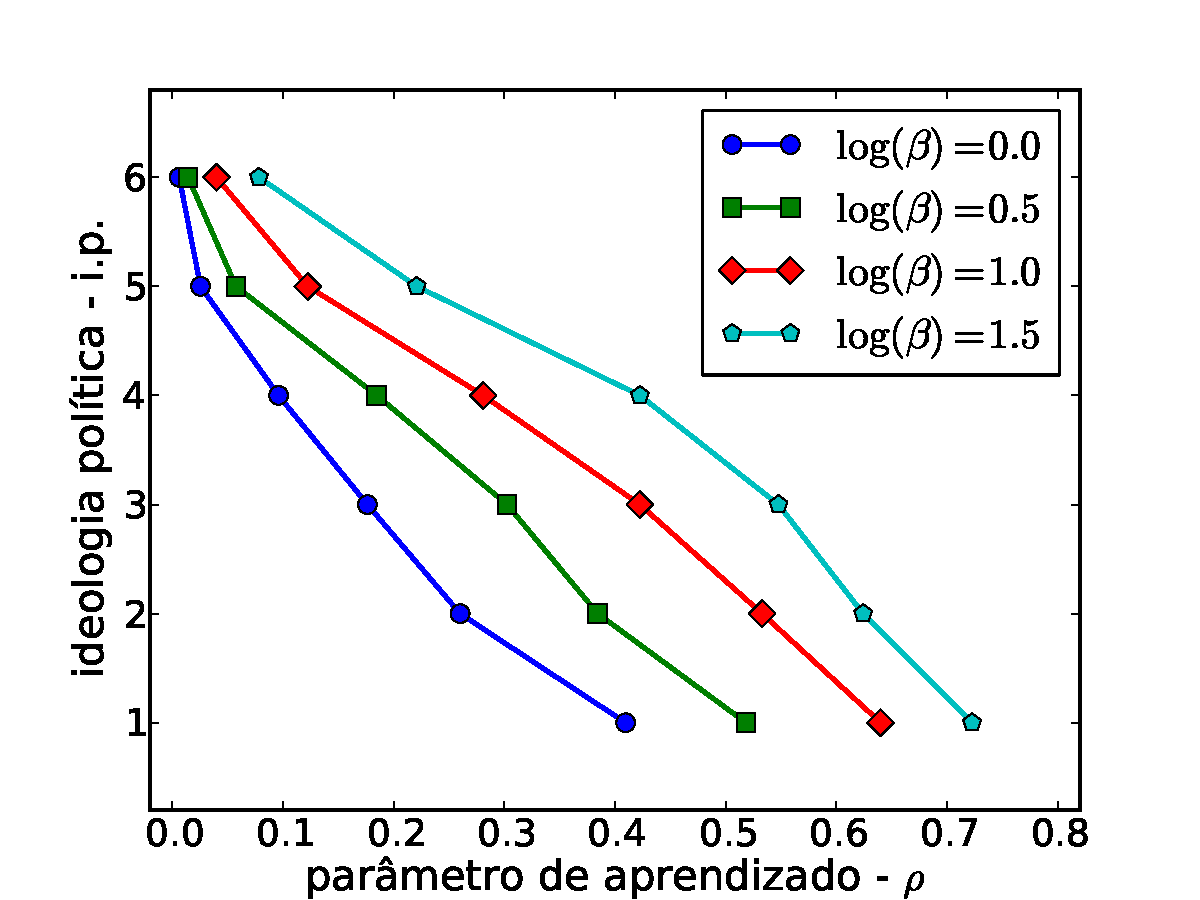
\includegraphics[scale=0.6]{Figures/pa-rho.pdf}
\caption{ Ideologia Política (pa= 1-Muito liberal, pa=7-Muito Conservador)
está correlacionada com  $\rho$, que é uma medida da diversidade moral
aprendida durante a Fase 1. Isso ocorre para uma grande variação do parâmetro
$\beta$ que avalia a pressão social.}
\label{fig:pa-rho}
\end{figure}

Já a figura \ref{fig:pa-rho} mostra como a ideologia Política (pa= 1-Muito
liberal, pa=7-Muito Conservador) está correlacionada com  $\rho$, que é
uma medida da diversidade moral aprendida durante a Fase 1. Isso ocorre
para uma grande variação do parâmetro $\beta$ que avalia a pressão
social. Percebemos claramente que quanto maior for o valor do parâmetro
$\rho$ mais os histogramas de opinião simulados se tornam similares aos
os histogramas experimentais de indivíduos liberais.

\newpage
\section{Diagrama Político}

O diagrama de fase é um dos instrumentos mais úteis para a caracterização dos
comportamentos em uma sociedade de agentes. Sua utilidade decorre do fato de
que os contornos de fase dividem regiões\footnote{No caso do diagrama de fase
apresentados na figura \ref{fig:diagfase} a linha preta é o único contorno de
fase} com comportamentos totalmente distintos.

\begin{figure}
    \centering
    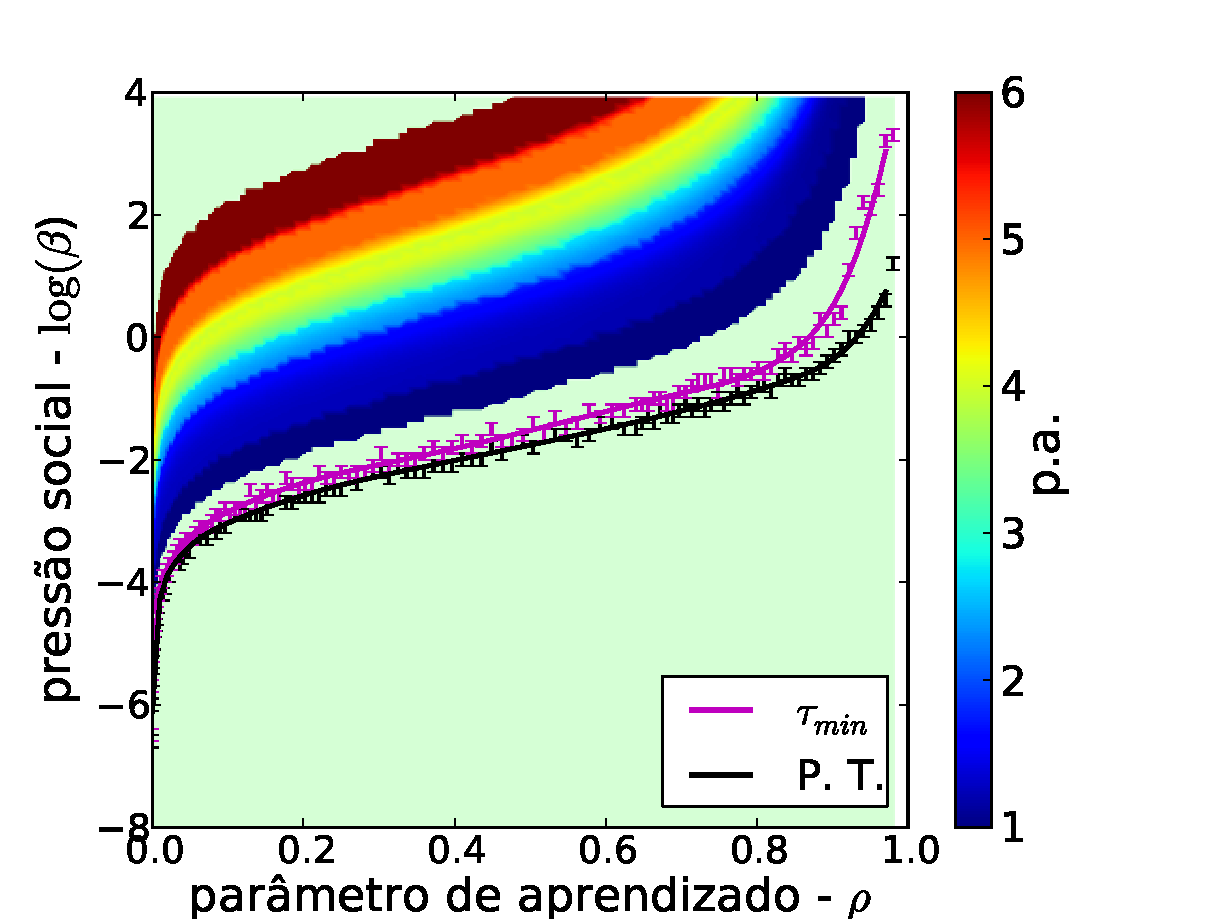
\includegraphics[scale=0.6]{Figures/padiag2.pdf}
    \caption{ 
        Diagrama de fase nos espaço, $\rho$ que mede a complexidade
        de socialização versus $\beta$ que mede a pressão social. As
        faixas coloridas representam sociedades de agentes que podem ser
        estatisticamente identificadas com grupos com diferentes ideologias
        políticas. A linha preta preta indica a transição de fase de
        uma sociedade totalmente desorganizada (a baixo da linha) para uma
        organizada. A linha magenta indica os parâmetros para os quais a
        sociedade tem os menores tempos de correlação.
    }
    \label{fig:diagfase}
\end{figure}

Na figura \ref{fig:diagfase} apresentamos o diagrama de fase nos espaço, $\rho$
que mede a complexidade de socialização versus $\beta$ que mede a pressão
social. As faixas coloridas representam sociedades de agentes que podem ser
estatisticamente identificadas com grupos com diferentes ideologias políticas. A
linha preta indica a transição de fase de uma sociedade totalmente
desorganizada (a baixo da linha) para uma organizada. A linha magenta indica os
parâmetros para os quais a sociedade tem os menores tempos de correlação. 


\newpage
\section{Conservadorismo e liberalismo de que?} %#{{{2

%falar denovo sobre a definição de conservadorismo de jost

O que o conservadorismo conserva? Se uma sociedade de agentes identificada como
conservadores ( pequeno $\rho$ ) se readaptassem a mudanças na sociedade mais
rapidamente do que sociedades liberais, nossa teoria deveria ser sumariamente
descartada. No entanto, o resultado de nossa teoria é que sociedades liberais se
readaptam mais rápido que sociedades conservadoras. 

Existem várias maneiras de se medir tempos de readaptação na sociedade que
trazem resultados qualitativamente equivalentes para a fase ordenada do
diagrama de fases. 

Uma maneira de medir tempos de readaptação foi introduzida em
\citep{Caticha2010}, onde depois que a distribuição de probabilidade
$P_S(h|\beta,\rho)$  de opiniões sobre um \textit{zeitgeist}, $\mc Z_{old}$ é
atingido, a dinâmica é reiniciada com os agentes discutindo um novo
\textit{zeitgeist} $\mc Z_{new}$. Com isso, um novo histograma de
opinião em relação ao novo \textit{zeitgeist} $P_t(h)$ é medido ao longo do
tempo. Medindo a distancia entre os histogramas 
\[
D(t) = \sum_{h\in bins} \left(P_t(h) - P_S(h|\beta,\rho)\right)^2
\]
somando a diferença quadrática entre as frequências de um conjunto de bins.
É esperado que existe um decaimento exponencial da distância ao londo do
tempo, $D(t) \propto \exp(-t/T)$, esse decaimento deve depender de um tempo de
adaptação médio $T$  que é função dos parâmetros $\rho$ e $\beta$. 

Uma segunda maneira de acessar essa informação é através do tempo de
decaimento da auto correlação da opinião dos agentes. Definimos a auto
correlação como a média temporal do produto entre as opiniões médias
dos agentes em dois tempos distintos subtraída do produto da média das
opiniões médias nesses tempos, ou seja,
\begin{align} 
    c(t) &=  \mean{m(t)m(t + t')} -  \mean{m(t)}\mean{m(t+t')} \nn
         &=  \frac{1}{t_{max} - t}\sum_{t'=0}^{t_{max}-t} m(t')m(t'+t)\nn
         & \quad \qquad  - \frac{1}{t_{max} - t}\sum_{t'=0}^{t_{max}-t} m(t')
         \times  \frac{1}{t_{max} - t}\sum_{t'=0}^{t_{max}-t}m(t'+t)
\end{align}
Essa grandeza também apresenta um decaimento exponencial que é dado na forma 
\[
c(t) \propto \exp \left( - \frac{t}{\tau} \right)
\]
sendo o tempo de relaxamento uma função dependente dos parâmetros
de socialização e pressão social, $\tau(\beta,\rho)$. 

Na figura \ref{fig:fasetempo}, mostramos o resultado de medidas de tempo de
correlação para diversas sociedades de agentes.  Podemos notar que existe
uma linha onde os tempos de autocorrelação divergem no meio de uma região
com baixos tempos. Essa linha ocorre exatamente na transição de fase e
é causada por um fenômeno comum em transições de fases conhecido como
\textit{desaceleração crítica}\footnote{tradução livre de:\\ \textit{Critical
Slowing Down.}} . A região abaixo dessa linha onde o tempo de correlação
permanece constante é a mesma onde a não existe organização social.

\begin{figure}
    \centering
    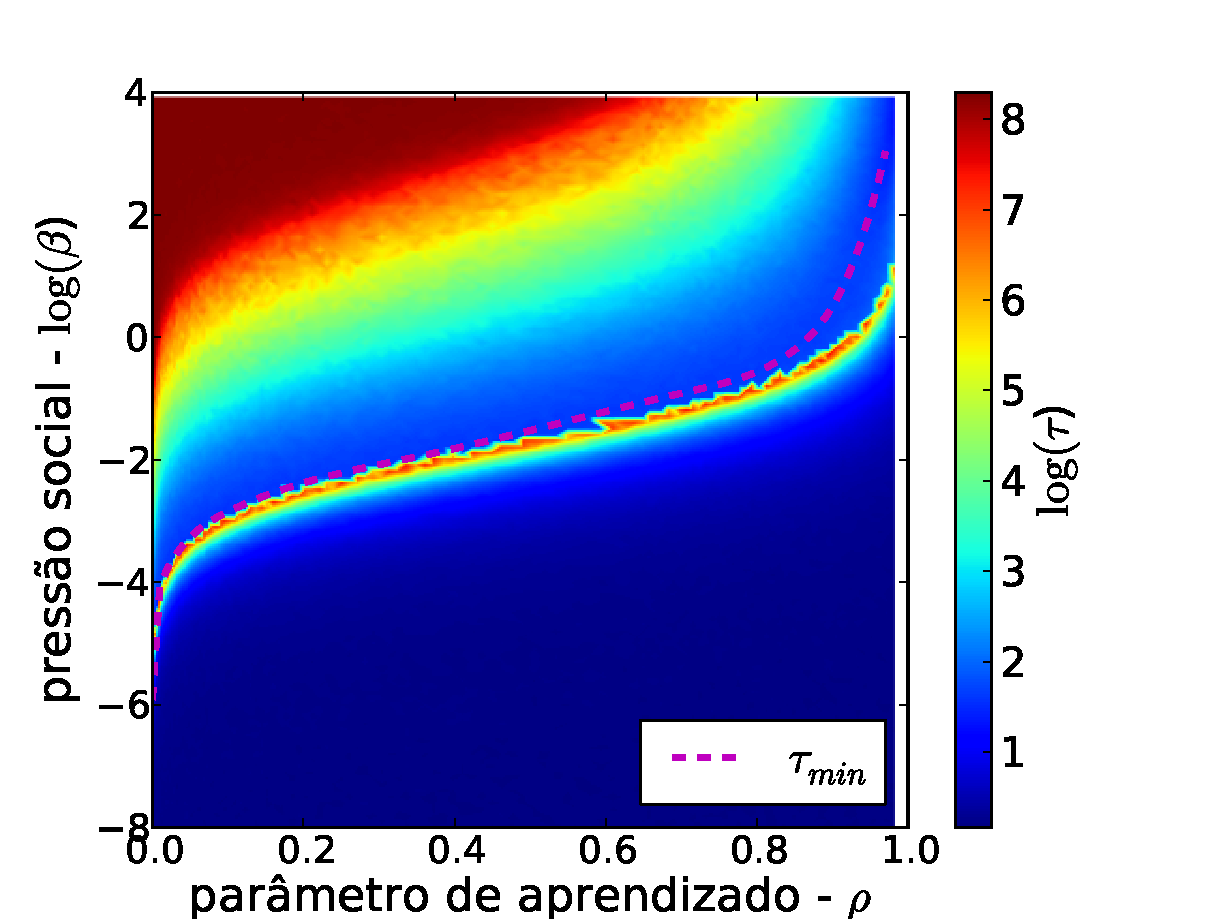
\includegraphics[scale=0.6]{Figures/tempocor_line.pdf}
    \caption{ 
        Figura com código de cores para o tempo de relaxação. Podemos
        observar que na linha de transição de fase o tempo de correlação
        diverge, esse fenômeno é conhecido como \textit{desaceleração crítica}. 
        Para sociedades de agentes identificadas como liberais o
        tempo de autocorrelação é menor do que para as sociedades de
        agentes identificadas como conservadores. Interessante notar que
        os sociedades identificadas como ultraliberais estão próximas da
        linha do tempo de correlação mínimo.
    }
    \label{fig:fasetempo}
\end{figure}


Acima da linha de transição de fase, observa-se que para um valor do
parâmetro $\rho$ fixo, a medida a pressão social aumenta o tempo de
correlação $\tau$ também cresce monotonamente.

Ainda é possível verificar que formato da região do diagrama de tempos de
correlação é semelhantes as faixas de cores que identificam as sociedades de
agentes com ideologias políticas. Com isso, podemos concluir que a filiação
política do indivíduo pode ser caracterizada pelo tempo de relaxação, e que
esse cresce a medida que andamos no espectro de filiação política no sentido
liberal conservador. É interessante notar que os sociedades identificadas
como ultraliberais estão próximas da linha do tempo de correlação mínimo.



\newpage
\section{Pressão Social} %#{{{2

O parâmetro de pressão social $\beta$ determina a escala de tolerância a
flutuações na função de custo psicológico $\mc E$, isto é, ele determina o quão
importante é em uma sociedade está em conformidade com seus pares. Dessa forma,
o parâmetro $\beta$ irá determinar, no estado estacionário do modelo, a escala
de flutuação das matrizes morais dos agentes entorno do \textit{zeitgeist}.

Assumindo que existe algum mecanismo, que não modelamos explicitamente, que
permite ao agente fazer um julgamento do ambiente social, podemos modelar
o efeito de ameaças externas ao grupo que o agente pertence considerando
aumentos no parâmetro de pressão $\beta$.

\begin{figure}
    \centering
    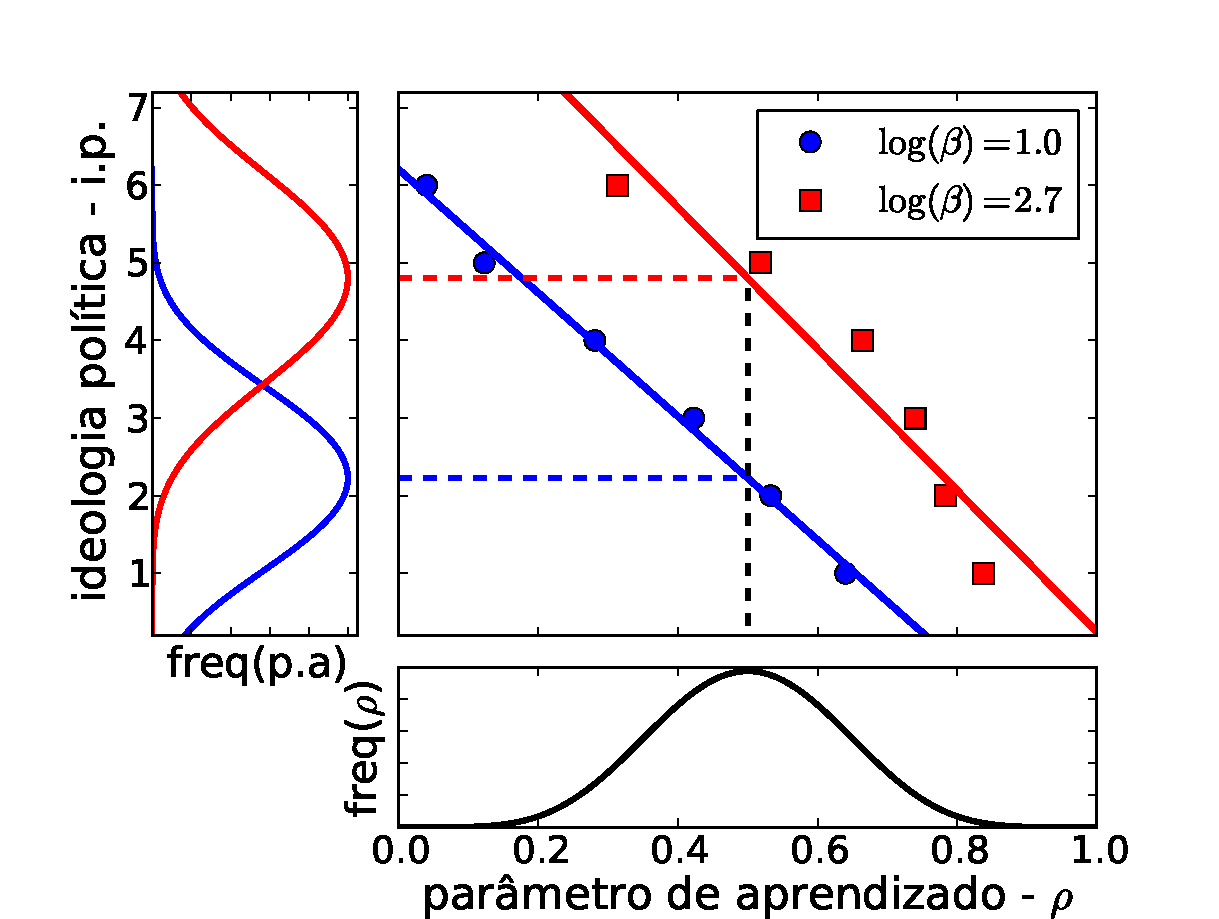
\includegraphics[scale=0.6]{Figures/dist-pa-rho.pdf}
    \caption{
        O proporção de  agentes conservadores muda com a pressão social.
        Se a população tem uma distribuição de encontros sociais apresentada na
        parte de baixo da figura a distribuição da filiação política
        resultante varia com a pressão social, como é mostrado na figura a
        direita.
    }
\label{fig:distpa}
\end{figure}

Supondo que existe uma distribuição de probabilidade para o número
de informação moral trocada entre os agentes na fase 1, ou seja, que
existe uma distribuição de probabilidade fixa para o parâmetro $\rho$
(figura \ref{fig:distpa}, gráfico em baixo), a distribuição de ideologia
política na população irá variar de acordo com o parâmetro $\beta$
(gráfico a esquerda). Como podemos ver pela figura \ref{fig:distpa}, para
uma sociedade com um alta pressão social os agentes se distribuirão com
mais concentração na parte conservadora do espectro político, e com menos
pressão social se concentra em torno da da parte mais liberal do espectro.

\begin{figure}
    \centering
    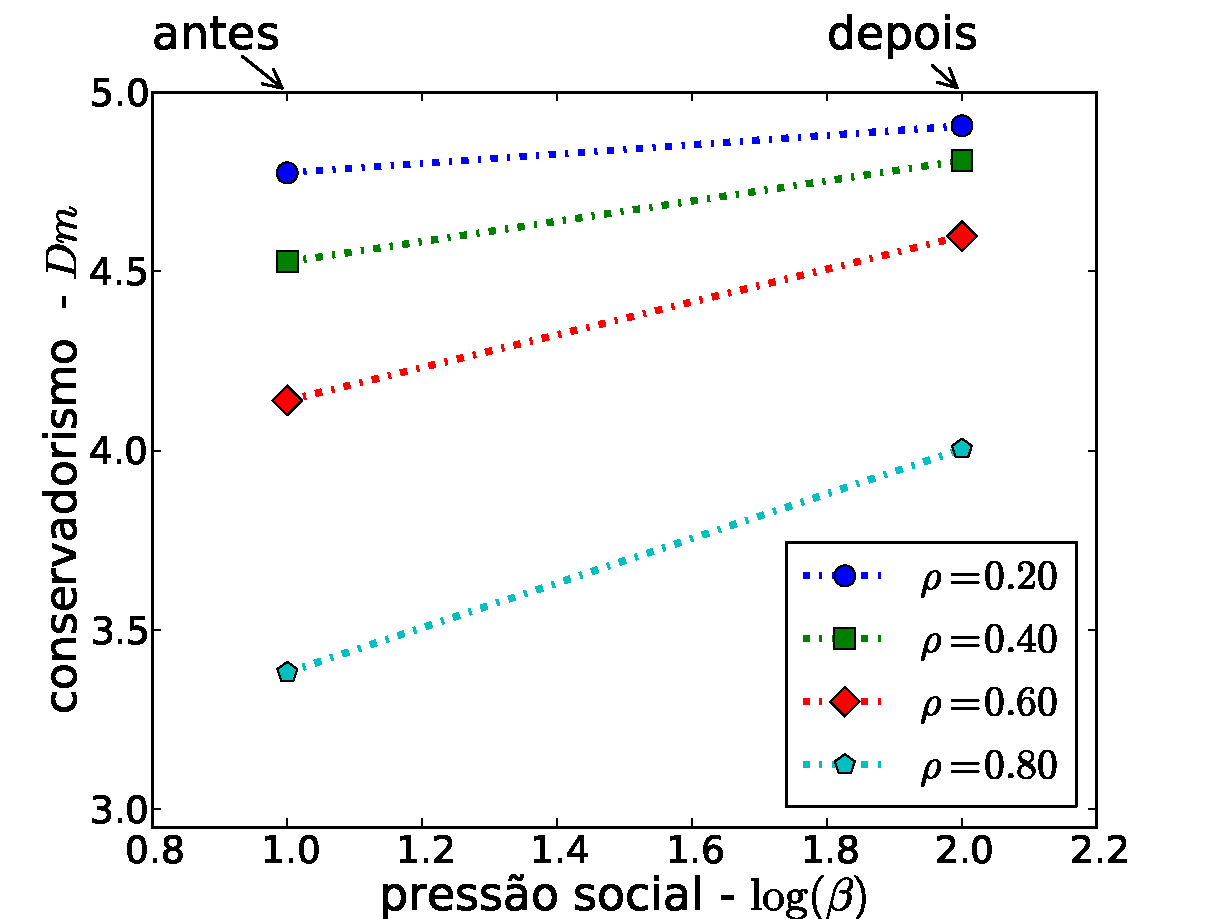
\includegraphics[scale=0.6]{Figures/threat.pdf}
    \caption{
        O número efetivo de dimensões morais para dois valores de pressão
        social, antes e depois de uma ameaça. Se ameaças acarretam em
        aumento da pressão social, a assinatura estatística de liberais se
        torna mais parecida com a de conservadores.
    } 
    \label{fig:threat}
\end{figure}

Outra maneiras de percebermos esse mesmo efeito é olhando para a variável
definida como número efetivo de dimensões morais usadas na sociedade. Isso é
feito multiplicando o número de dimensões morais $d_m = 5$ pela opinião média
dos agentes em relação ao \textit{zeitgeist}. Na figura \ref{fig:threat}
observamos o efeito de crescimento da dimensão moral efetiva da sociedade com
diferentes vares de $\rho$ no caso de um aumento na pressão social devido a uma
ameaça. 

\newpage
\section{Detalhes computacionais} %#{{{2

Todos os resultados de simulação descritos nesse capítulo, assim como os
gráficos \ref{fig:ordem} e \ref{fig:chi} do capítulo anterior, foram obtidos
através da simulação de  sociedade com 400 agentes dispostos sobre uma rede
do tipo Barabasi-Albert com um número médio de 20 vizinhos.  Escolhemos esse
número de vizinho pois evidências experimentais \cite{Trusov2010} sugerem que
o número de parceiros sociais  relevantes de uma pessoa está entre 18 e 22. 
A dependência com a estrutura da rede foi estudada no contexto do modelo
proposto por Caticha e Vicente\citep{Caticha2011a} no apêndice
\ref{sec:deppar} e na dissertação de metrado de Jericó \cite{Jerico2012}.
Para um revisão sobre grafos complexos e suas aplicações nos mais diversos
contextos recomendamos ao leitor a referência \citep{Albert2002}.

Cada ponto dos gráficos apresentados foram resultados de médias de pelo
menos 800 configurações de Monte Carlo independentes, dependendo do tempo de
correlação da simulação. As simulações foram feitas em 33 computadores
de quatro núcleos e velocidade de processamento entre 2.4 e 2.8 Ghz. Foram
gastos aproximadamente 8 dias de simulação contínua em todos os núcleos.
